\section{Input Medium Selection}
\label{sec:medium-selection}

The first step in this project was to establish the best method for a student to interact with the application. As seen in \cref{sec:prior-research} a lot of different mediums for OMR have been tried over the years, however which one would be most suitable for a student to use wouldn't necessarily correlate with which was best for quality of scanning, speed of analysis etc.

\subsection{Flat Bed Scanner}

The most simple of all the input methods, this would involve a student writing on a sheet of manuscript paper, then using a flat bed scanner (the type commonly found as a standalone device and in multi-function printers) to input the sheet into the computer. This method allows for a scan with high and consistent light levels (minimising noise and light-dependent artefacts), minimal distortion due to paper curvature (as the scanner usually flattens the sheet) and a high resolution end image, typically 300-600dpi.

The application would process the sheet using traditional OMR techniques and then provide feedback to the student. This technique would therefore require ownership of both a scanner and a computer on which to install and run the application. Alternatively, the student could upload the scanned image to a web based service for analysis, removing the need to install software.

\subsection{Photograph/Camera}

\todo[inline,color=red]{Implementation - Photo/Camera}

Total free for all, colours and light levels vary, extraction from background, resolution variable, noise variable

Reference `Project 8 Final Report'

\subsection{Gestures}
\todo[inline,color=red]{Implementation - Gestures}

Use gestures combined with classification (see book and some papers).
Good for classifying individual entities but more like the old palm tablets, usually one note at a time

\subsection{Tablet Input}
\todo[inline,color=red]{Implementation - Tablet Input}

Finger or stylus work well tends to depend on the child, finger often felt more natural

\begin{figure}[h!]
    \centering
    \begin{subfigure}[b]{.4\linewidth}
        \centering
        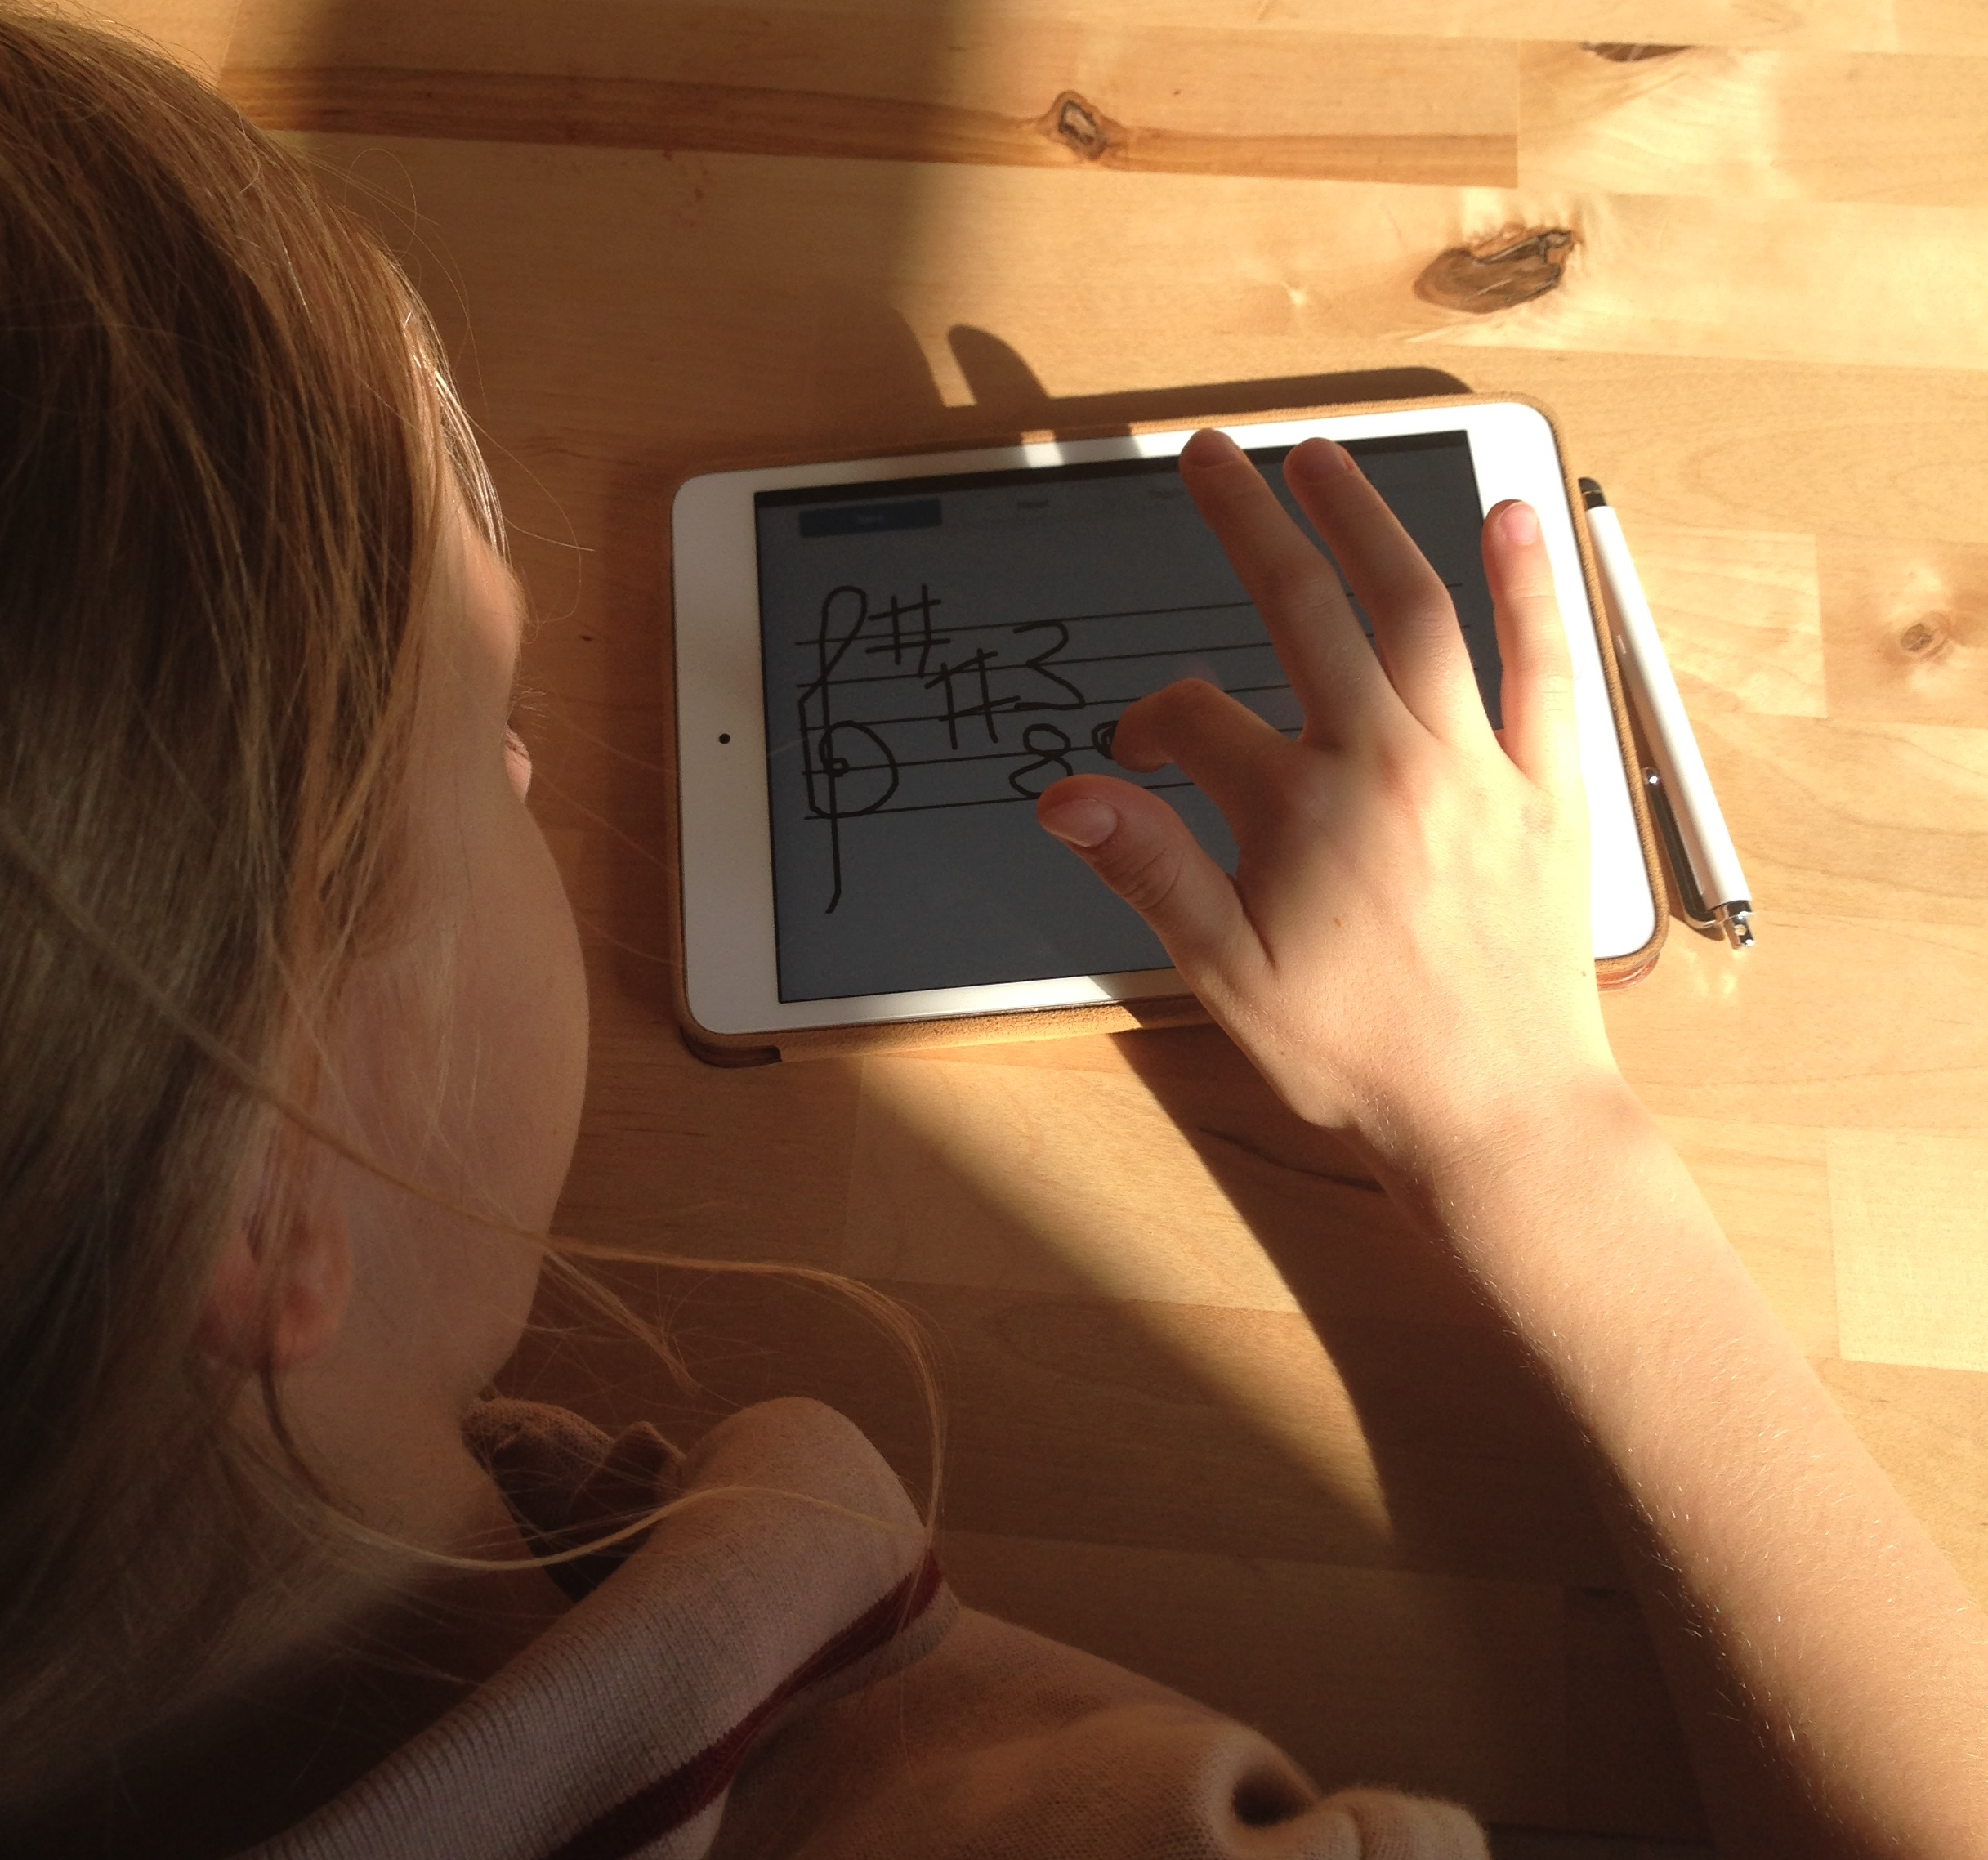
\includegraphics[height=6cm]{gfx/photos/user-finger.jpg}
        \caption{Using their finger}
    \end{subfigure}
    \begin{subfigure}[b]{.4\linewidth}
        \centering
        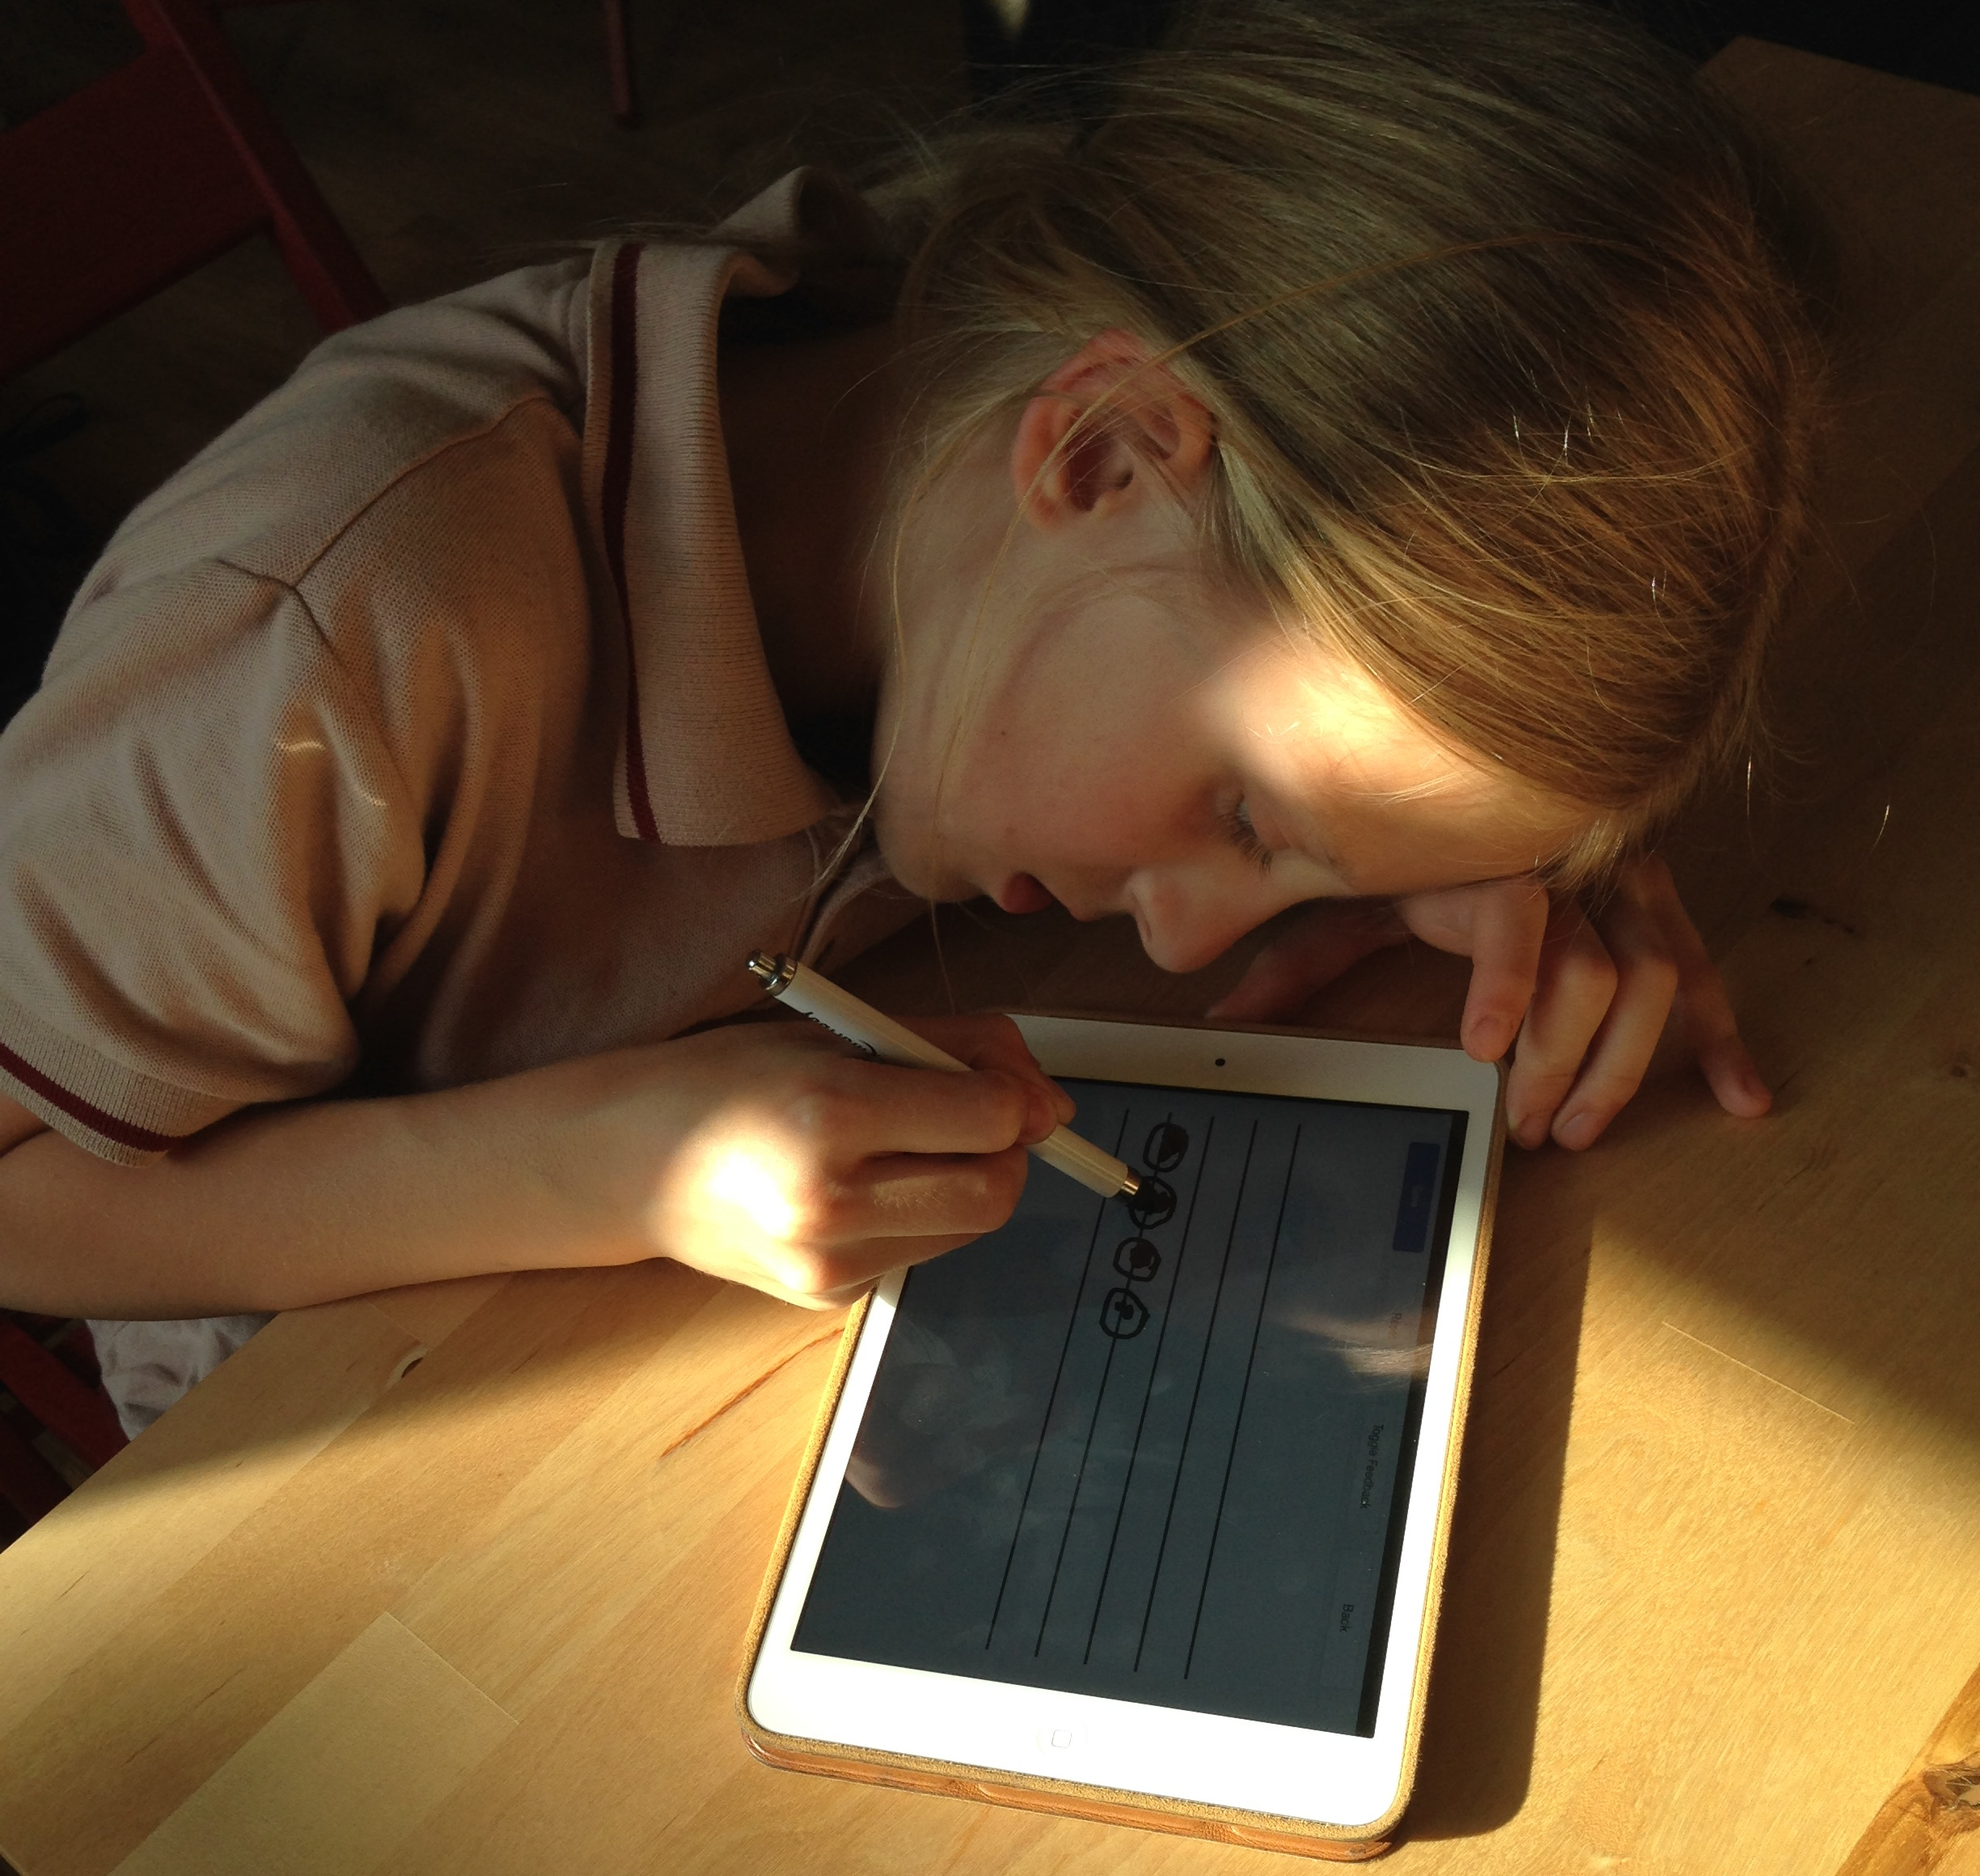
\includegraphics[height=6cm]{gfx/photos/user-stylus.jpg}
        \caption{Using a stylus}
    \end{subfigure}

    \caption{Examples of a student trying different tablet input methods}
\end{figure}

Chose this method in the end
